\documentclass[12pt]{article}

% page packages
\usepackage[left=1.5cm,right=2.5cm,top=2cm,bottom=3.5cm,paperwidth=10.5cm,paperheight=15.5cm]{geometry}
\usepackage{pgfpages}
\usepackage[a4,cross]{crop}
\usepackage{wallpaper}

% content packages
\input GoudyIn.fd
\newcommand*\initfamily{\usefont{U}{GoudyIn}{xl}{n}}
\usepackage{chancery}
\usepackage[T1]{fontenc}

% page defs
\pgfpagesdeclarelayout{christmas}{
    \edef\pgfpageoptionheight{\the\paperheight}
    \edef\pgfpageoptionwidth{\the\paperwidth}
    \edef\pgfpageoptionborder{0pt}
}{  \pgfpagesphysicalpageoptions{
        logical pages=2, physical height=29.7cm, physical width=21.0cm
    }\pgfpageslogicalpageoptions{2}{
        border shrink=\pgfpageoptionborder, resized width=10.5cm, resized height=15.5cm,
        center=\pgfpoint{.25\pgfphysicalwidth}{.5\pgfphysicalheight}
    }\pgfpageslogicalpageoptions{1}{
        border shrink=\pgfpageoptionborder, resized width=10.5cm, resized height=15.5cm,
        center=\pgfpoint{.75\pgfphysicalwidth}{.5\pgfphysicalheight}
    }
}\pgfpagesuselayout{christmas}
\pagenumbering{gobble}

\newcommand{\h}[1]{\textcolor{red!70!black}{#1}}

\begin{document}
%% COVER %%
%\ThisCenterWallPaper{1}{china-bottle-4-16003}
\ThisCenterWallPaper{1}{china-vase-3-16002}

\phantom{just a placeholder}
\newpage\null\newpage

%% CONTENT %%
\ThisCenterWallPaper{1}{u71}

% flower
\begin{figure}
    \vspace*{-0.5cm}
    \centering
    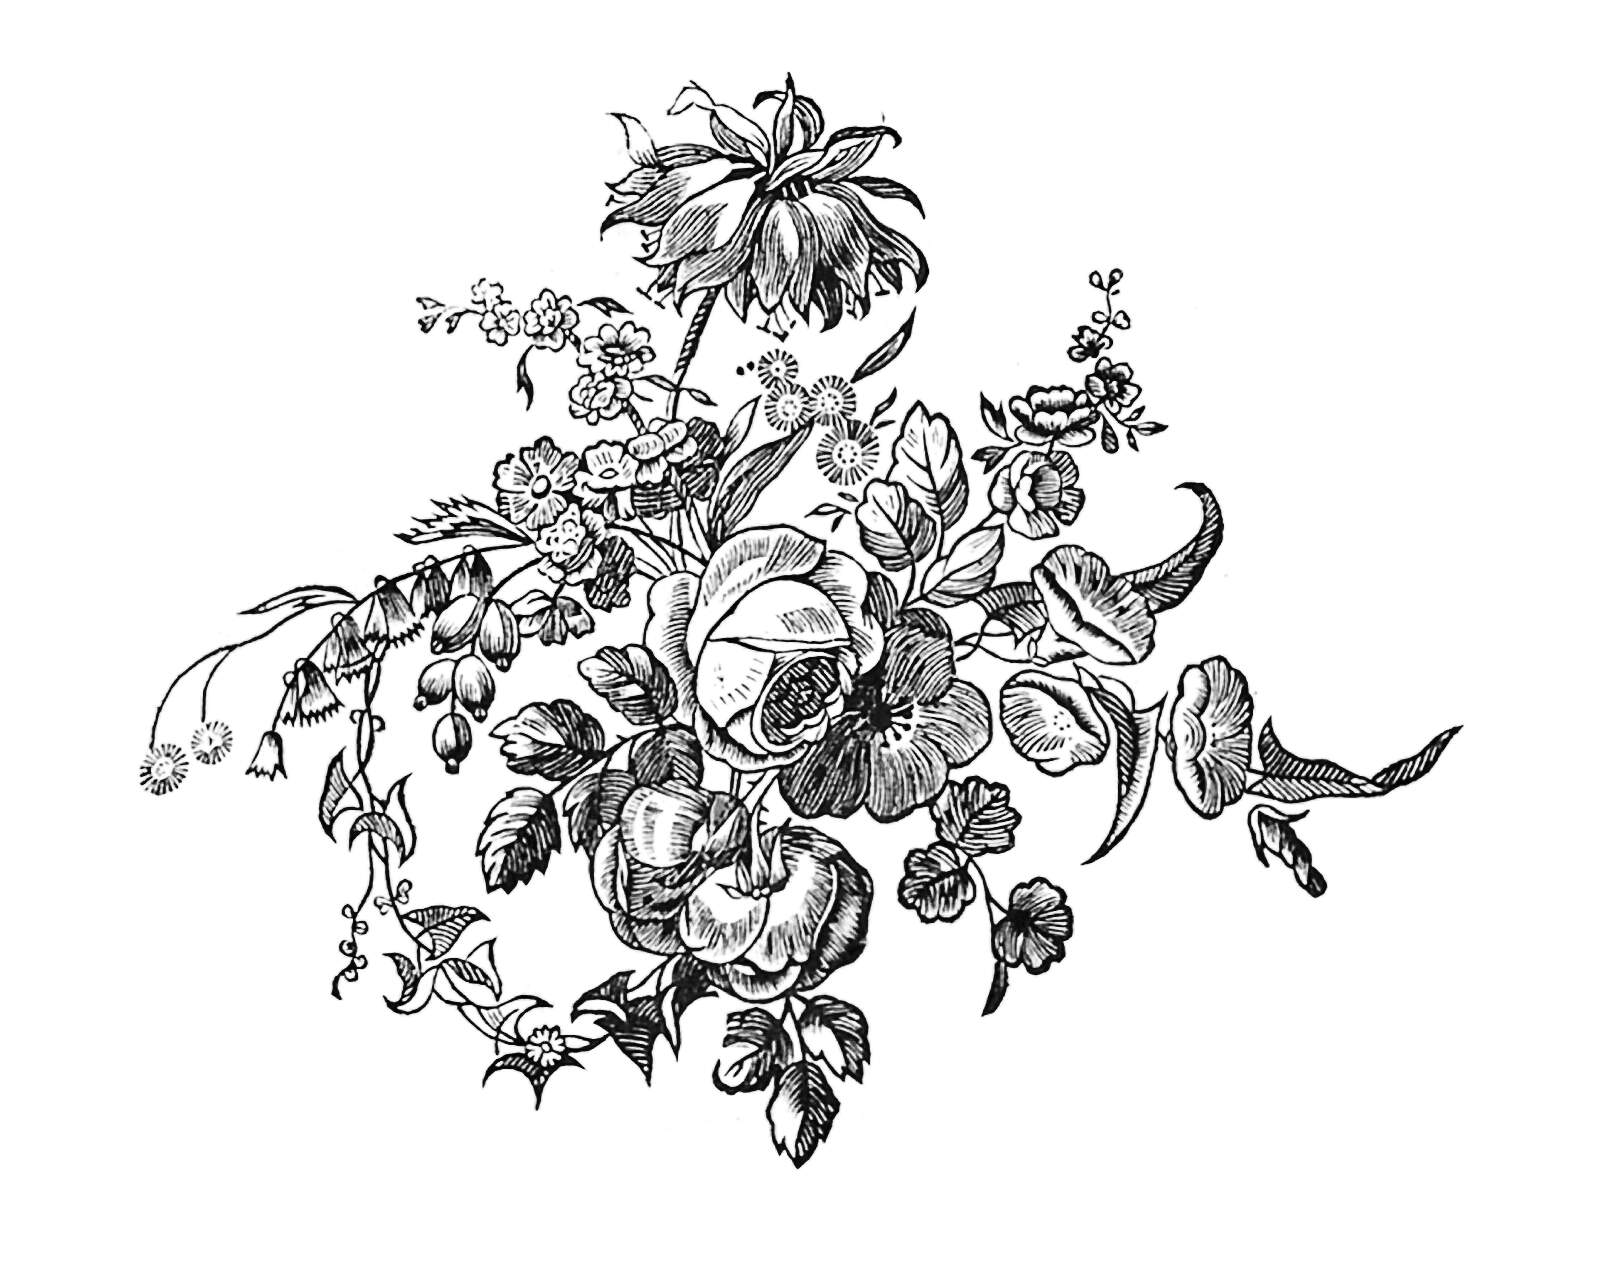
\includegraphics[width=0.5\textwidth]{gille-flowers-1600}
\end{figure}
\smallskip

% words
\begin{center}
Dear \h{M}o, \\
I wish you a\\
\huge{\textsc{\h{H}appy \h{V}alentine}}
\end{center}
\bigskip
Thank you for all these years, \\
and even more for the years to come.
\\

% signature
\vfill
\begin{flushright}
Love,\\
\h{H}o\\[4pt]

\normalfont\initfamily
\fontsize{12mm}{12mm}\selectfont \h{HS}
\end{flushright}

\end{document}

%Source
%- cover https://www.oldbookillustrations.com/illustrations/china-bottle-4/
%- border https://www.fromoldbooks.org/WilliamMorris-KelmscottChaucer/pages/483-Troilus-and-Criseyde-II-In-May-outer-border/
%- flower https://www.oldbookillustrations.com/illustrations/gille-flowers/